\chapter{Accès utilisateurs}

    Afin de filtrer et maîtriser les informations circulant sur le site, ainsi que pour fidéliser les visiteurs les plus assidus, nous construisons un espace membre permettant aux visiteurs de créer et/ou de se connecter pour avoir accès à des fonctionnalités supplémentaires du site.

    \section{Inscription ou Connexion sur DodoCiné}

        Les visiteurs du site peuvent se connecter à tout moment, en utilisant le bouton \erd{Connexion} situé à droite dans la barre de navigation. 


        \begin{figure}[!ht]
            \centering
            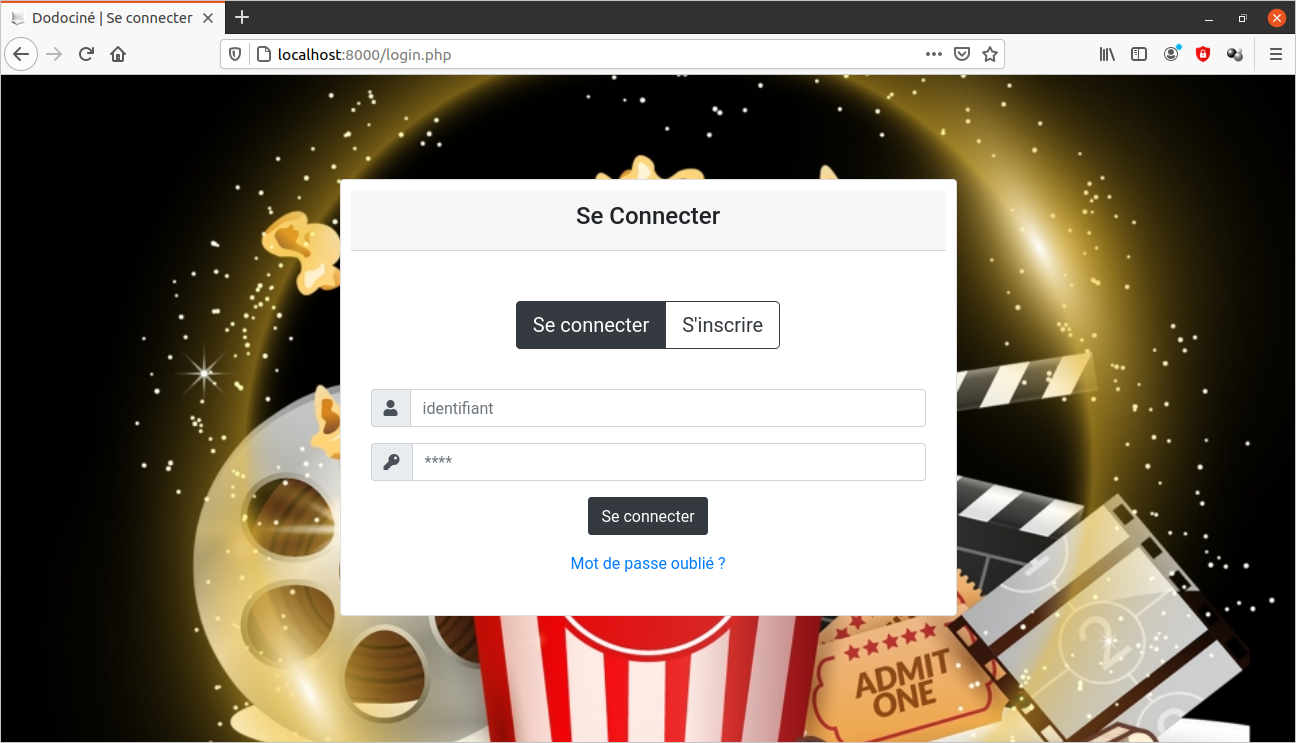
\includegraphics[width=15cm]{img/connexion.png}
            \caption{Page de connexion/inscription sur DodoCiné}
        \end{figure}

        \medskip
        Si le visiteur ne possède pas encore son propre compte, il peut s'inscrire en se rendant sur l'onglet \erd{S'inscrire} et remplir un formulaire d'inscription. Pour plus de confidentialité, on demande au futur membre de choisir un pseudonyme: ce pseudonyme servira à l'identifier sur le site tout au long de sa visite auprès des autres membres du site.

        \bigskip
        \boiteinfo{Fichiers utilisées pour cette partie du site}{
            \begin{itemize}
                \item \f{login.php} qui est la page appelée lorsque l'on clique sur le bouton "Connexion"
                \item \f{elements/login-form.php} et \f{elements/signup-form.php} contiennent les formulaires de connexion et d'inscription. Nous avons fait le choix de les écrire dans des fichiers séparés avant d'améliorer la visibilité de notre fichier \f{login.php}.
                \item \f{static/css/login.css} 
                \item \f{static/js/login.js} est le script JQuery/Javascript permettant d'ajouter du dynamisme à la page.
                \item \f{login-response.php} contient le script PHP "pur" qui répond aux demandes Ajax du fichier \f{static/js/login.js} 
            \end{itemize}
        }      

        \bigskip
        \subsection*{Présentation de la page}

            En nous inspirant des dernières tendances, nous avons construit une unique page dans laquelle il est possible au choix de se connecter ou de s'inscrire. Le passage d'un formulaire à l'autre se fait via une fonction JQuery qui, selon le bouton sélectionné cache un formulaire et fait apparaître le second.


        \bigskip
        \subsection*{Vérification des informations renseignées dans les formulaires}

            Afin d'offrir une meilleure expérience aux utilisateurs du site, nous avons fait le choix d'effectuer toutes les vérifications d'informations à l'aide de Ajax et d'un script PHP. Lorsque l'utilisateur appuie sur le bouton \erd{S'enregistrer} ou \erd{S'inscrire}, nous effectuons un appel Ajax qui appelle à son tour notre script PHP \f{login-response.php} par la méthode POST. A l'intérieur de ce script, nous vérifions tout d'abord si tous les champs sont bien renseignés puis si les informations entrées sont correctes vis-à-vis du contenu de la base de données (en particulier la table \erd{users} ici). Si des erreurs surviennent, celles-ci sont renvoyés afin que l'on puisse afficher une indication à l'utilisateur. A l'inverse, en l'absence d'erreur l'utilisateur est connecté et est renvoyé sur la page d'accueil du site. 

            \begin{figure}[!ht]
                \centering
                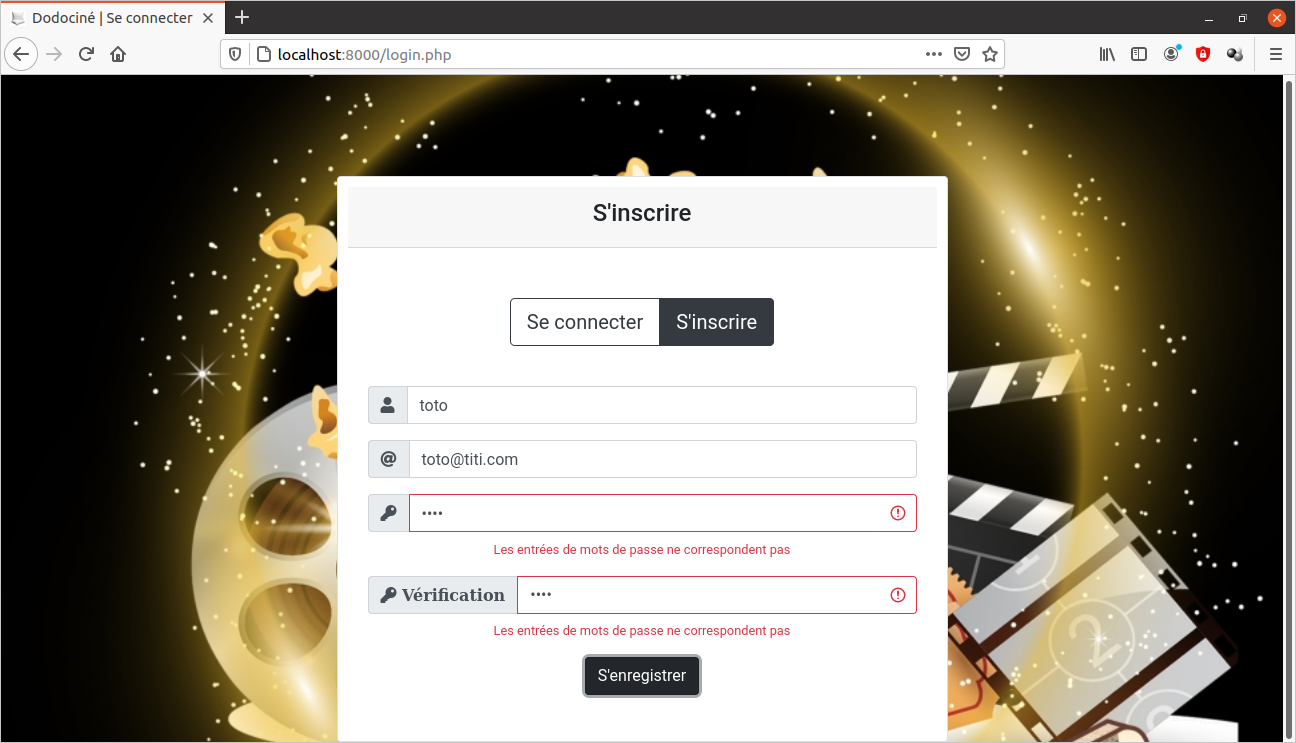
\includegraphics[width=12cm]{img/erreur-form.png}
                \caption{Affichage d'indications d'erreurs sur les formulaires d'inscription et de connexion}
            \end{figure}

            \medskip
            Une fois connecté, le visiteur peut remarquer que son pseudonyme se substitue au bouton de connexion dans la barre de navigation. En cliquant dessus, il peut alors accéder à son espace personnel\footnote{voir plus loin} ou tout simplement se déconnecter.


            \bigskip
            Problèmes rencontrés lors de la programmation:
            \begin{itemize}
                \item Suite à l'utilisation d'AJAX pour passer nos requêtes, nous constatons que l'utilisation de la fonction "header('Location: index.php')" ne fonctionne plus. Après recherches dans la documentation de PHP, nous avons découvert que cela était dû au fait que cette fonction ne fonctionne que si aucun code html n'est encore affiché sur la page. Pour effectuer cette redirection, nous choisissons dorénavant d'utiliser la méthode Javascript "window.location.replace(url\_redirection);"

                \item Lors de l'écriture d'un script JQuery, l'utilisation d'un argument {\itshape event} dans la fonction {\itshape \$(document)\$.ready(function(event) \{\});} nécéssitait l'appel de la méthode {\itshape event.preventDefault();} afin d'empêcher le rechargement automatique de la page. Cependant, si {\itshape function} ne prend aucun argument, alors l'utilisation de la méthode n'est plus indispensable et la page ne se recharge pas. 
            \end{itemize}


    \section{L'espace membre associé à un compte}

        \begin{figure}[!ht]
            \centering
            \includegraphics[width=15cm]{img/espace-membre.png}
            \caption{Espace Membre/Paramètres daans DodoCiné}
        \end{figure}


        Dans cet espace, l'utilisateur peut modifier les paramètres de son compte, tel que changer son mot de passe, son email, ou même se désinscrire (entrainant la suppression de son compte), ou bien accèder plus rapidement aux messages et aux notes qu'il a postés sur le site.

        \bigskip
        \boiteinfo{Fichiers utilisées pour la partie 'espace membre'}{
            \begin{itemize}
                \item \f{parameters.php} qui est la page principale.
                \item architecture des onglets de la page:
                    \begin{itemize}
                        \item \f{parameters-config.php} pour modifier ses informations personnelles
                        \item \f{parameters-fav.php} pour accéder à sa liste de films favoris
                        \item \f{parameters-rating.php} est l'onglet rappelant à l'utilisateur les notes qu'il a donnés à différents films ainsi que ses derniers messages dans différents forum.

                        \medskip
                        Chacun des onglets est caché/affiché à l'aide de fonctions définies dans le script JQuery/Javascript.
                    \end{itemize}
                \item \f{static/css/parameters.css} 
                \item \f{static/js/parameters.js} est le script JQuery/Javascript permettant d'ajouter du dynamisme à la page.
                \item \f{parameters-response.php} contient le script PHP "pur" qui répond aux demandes Ajax du fichier \f{static/js/login.js} 
            \end{itemize}
        }  

        \subsection{Rappels des notes et des messages postés}


            Nous proposons à l'utilisateur, dans l'onglet "mes notes et messages", de retrouver quelques statistiques sur ces interventions sur le site:
            \begin{itemize}
                \item le nombre de messages postés
                \item le nombre de films notés
                \item la moyenne des notes données
            \end{itemize}

            De plus, il peut voir les derniers messages qu'il a postés et avoir un lien direct pour rejoindre le fil de discussion et continuer à échanger avec d'autres utilisateurs. 

            \smallskip
            Les messages sont présentés dans un tableau, avec le début du message ainsi que le film auquel se rapporte le message. En cliquant sur le nom du film, l'utilisateur retourne directement sur sa fiche et a accès au forum. Nous faisons le choix de n'afficher que les 5 derniers messages et ce pour éviter, le cas échéant, l'affichage d'un nombre trop important de messages.  


        \subsection{Paramètres du compte}

            \begin{figure}[!ht]
                \centering
                \includegraphics[width=15cm]{img/param-config.png}
                \caption{Section Paramètres du compte dans l'espace membre}
            \end{figure}

            Dans cette section, nous avons créé deux formulaires distincts, l'un permettant de modifier le mot de passe du compte et le second, l'email. Nous avons construit ces formulaires et les appels associés de la même façon que pour la connexion/inscription d'un utilisateur: à l'aide d'Ajax, nous vérifions les erreurs potentielles entrées par l'utilisateur et les affichons le cas échéant. En cas de succès, une fenêtre modale apparait pour indiquer que les informations ont bien été modifiées.

            \medskip
            Cette fenêtre modale est un composant intégré du framework Bootstrap, ce qui nous permet de l'utiliser de façon simplifiée sans nous inquiéter de la partie Javascript qui est pré-programmée. De plus, ces "modals" sont très facilement modulables ce qui les rend très simples d'utilisation.  

            \medskip
            Enfin, le bouton \erd{Suppression} permet à l'utilisateur, s'il le souhaite, de supprimer de façon définitive son compte. En cas de sélection, le compte est supprimé, et les informations concernant cet utilisateur seront supprimées. Néanmoins, les notes données, ainsi que les messages postés sont conservés car devenus publics.

        \subsection{Favoris}

            Nous avons souhaité ajouter une petite fonctionnalité à notre site en offrant à nos utilisateurs la possibilité de "sauvegarder" les films qui l'intéressent, par exemple pour créer une liste de films à visionner, ou de films qui lui plaisent particuièrment. Pour cela, il lui suffit de cliquer le bouton "Ajouter aux favoris" disponible sur la fiche d'un film. Tous les films ajoutés sont ensuite présentés dans la section \erd{Mes Favoris} de son espace Membre.
